For each patient we hereby present a performance result both for
classification and regression.

For classification, the performance index is the \emph{weighted}
percentage of correctly guessed labels, that is, the average of the
percentages for each label $i$, divided by the number of labels $i$ in
the testing set. This measure, as opposed to the more standard ratio
of correctly guessed labels, has the advantage of adjusting the
importance of each label according to how often it appears in the
testing set. For example, in general there are more $0$ labels in any
testing set than other labels, since $0$ appears both at the beginning
of the experiment and in-between the grasps, as it represents
rest. Therefore this label must be weighted \emph{less} than the
others, since it is more easily found in the testing set.

For regression, the performance index is the standard Pearson
correlation coefficient evaluated between the predicted force signal
and the real one (remember that we work in real-time, so that this
measure of correlation really is a measure of temporal
correlation). The choice of the correlation coefficient, as opposed to
the more standard mean-square error, is suggested by a practical
consideration: when driving a prosthesis, or even a non-prosthetic
mechanical hand, we are not interested in the absolute force values
desired by the user/subject, since mechanical hands usually cannot
apply as much force as human hands do, for obvious safety
reasons\footnote{or, e.g., in teleoperation scenarios, they could be
able to apply \emph{much more} force than a human hand can.}. We are
rather concerned about getting a signal which is \emph{strongly
correlated} with the patient's will.

As is standard in machine learning, each data set was split in $5$
folds and cross-validation was performed on it; this makes the
evaluation robust against the problem of over-fitting. We employed a
well-known freely available SVM package, \emph{libsvm} v2.83
\cite{ChangL01}, in the Matlab wrapped flavour, with a Gaussian
kernel. This particular kind of SVM requires setting two
\emph{hyperparameters}, called $\gamma$ and $C$, which were found by
grid search using the aforementioned performance indexes.

Table \ref{tab:results} shows the main results obtained by the SVMs.

\begin{table}[!ht] \centering
  \caption{Classification/regression performance for each subject
    (row) and modality (column).}
  \begin{tabular}{|c|r|r|r|}
    \hline
                & Imitation & Bilateral & Mirror \\
    \hline
    Subject $1$ & $93.09\%$ / $0.96$ & $90.39\%$ / $0.95$ & $82.48\%$ / $0.93$ \\
    Subject $2$ & $88.70\%$ / $0.86$ & $95.90\%$ / $0.96$ & $96.09\%$ / $0.94$ \\
    Subject $3$ & $85.55\%$ / $0.83$ & $94.99\%$ / $0.93$ & $93.57\%$ / $0.93$ \\
    \hline
  \end{tabular}
  \label{tab:results}
\end{table}

The first consideration is that for each subject, at least one
modality produces excellent results, both in classification and
regression. Subject $1$ works best by imitation, whereas subjects $2$
and $3$ exhibit best results via bilateral action and mirror-box. If
we consider the best modality for each subject, we get an average
classification accuracy of $94.72\%$ and an average regression
correlation of $0.95$. Essentially the system can predict everything,
as is apparent from Figure \ref{fig:examples} in which a comparison is
shown between bits of real target labels and values and the
corresponding guessed targets.

\begin{figure*}[!ht] \centering
  \begin{tabular}{ccc}
    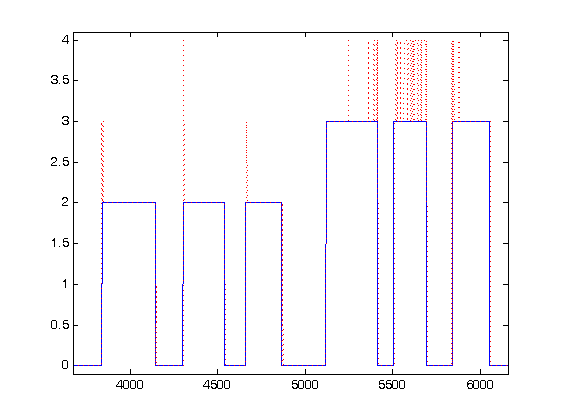
\includegraphics[width=0.3\textwidth]{figs/example1} &
    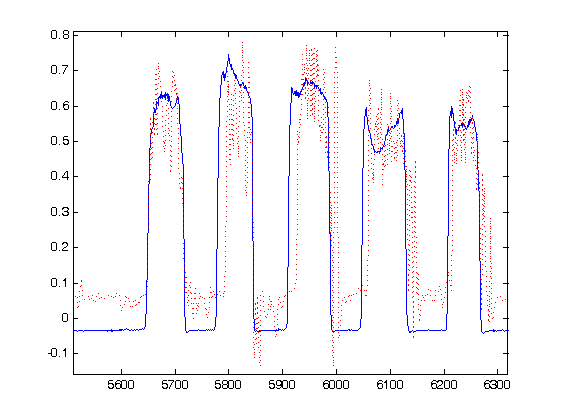
\includegraphics[width=0.3\textwidth]{figs/example2} &
    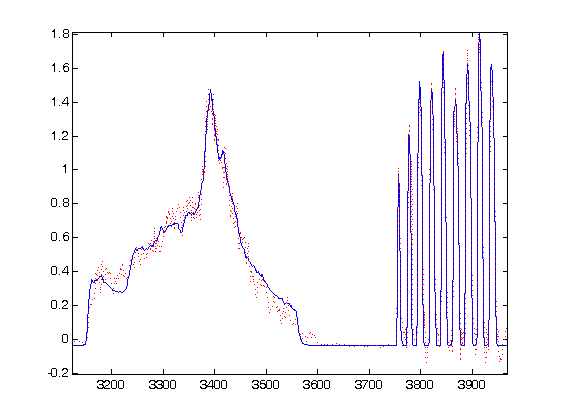
\includegraphics[width=0.3\textwidth]{figs/example3} \\
    $(a)$ & $(b)$ & $(c)$ \\
  \end{tabular}
  \caption{comparing true and guessed labels $(a)$ and force values
    $(b)$ and $(c)$. Notice, in panel $(a)$, that labels
    $3$ (pinch grip) are often mistaken for labels $4$ (tripodal
    grip). Notice also, especially in panel $(c)$, the almost perfect
    correlation between force and guessed force, both during a slow
    buildup/release and during quick applications of force.}
  \label{fig:examples}
\end{figure*}

Consider the Figure, panel $(a)$: the major problem seems that of
pinch grips which get mistaken for tripodal grips, and this is
intuitively clear, since these two types of grips are quite similar
from an anatomical point of view. This fact is corroborated by the
fact that (consider Figure \ref{fig:PCA} again, pink and black dots)
the two grips lie, almost consistently, in the same regions of the
$2$-dimensional PCA-transformed input space.

\begin{figure*}[!ht] \centering
  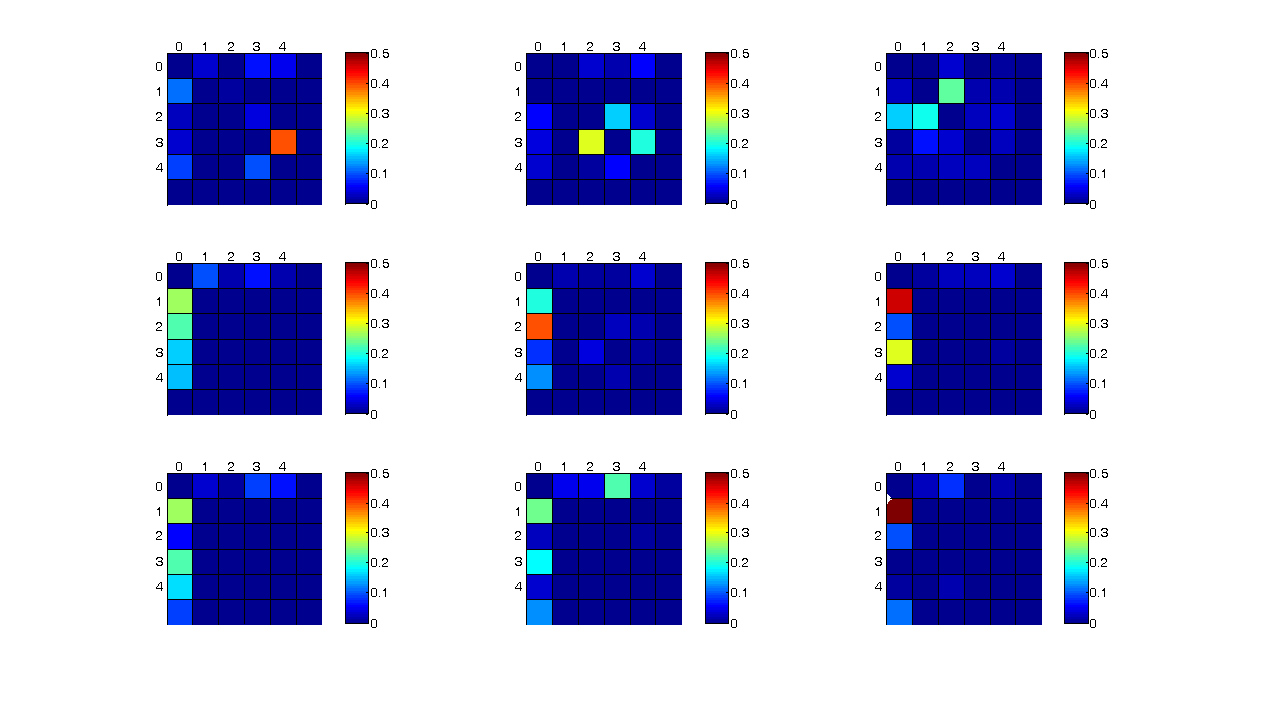
\includegraphics[width=\textwidth]{figs/confusion}
  \caption{confusion matrices for each subject / modality
    pair. Subjects are on each row, modalities are on each column. In
    each matrix $C$, the entry $C_{ij}$ denotes the fraction of labels
    $i$ which have been mistaken for $j$ over the total mistaken
    labels of that particular pair. The diagonals of the matrices are,
    therefore, identically zero.}
  \label{fig:confusion}
\end{figure*}

Actually, the confusion matrices related with each subject / modality
pair (see Figure \ref{fig:confusion}) do not confirm this feeling:
most mistakes in classification involve label $0$, both in the sense
that $0$ is mistaken for something else and vice-versa (consider the
first row and first column of each matrix). This happens especially
(consider rows $2$ and $3$ of the Figure) for subjects $2$ and $3$,
whereas subject $1$ presents more uncertainty as far as other
confusion pairs are concerned. This phenomenon is also clearly
justifiable, since misclassifications involving label $0$ (the
``rest'' position) happen at the onsets / endings of grips. A simple
buffering strategy (i.e., considering a few samples before switching
category) would probably suffice to eliminate this problem.

As far as regression is concerned, consider now Figure
\ref{fig:examples}, panels $(b)$ and $(c)$. If we neglect a
high-frequency oscillation, the guessed force values are essentially
replicating the true values --- again, there are different offsets,
but this is a direct result of choosing \emph{maximum correlation} as
the performance index. The signals in the Figure could easily be used
in practice after a simple linear trasnformation. Notice in particular
(panel $(c)$) how the system is smoothly able to correctly guess both
low-frequency (left-hand side) and high-frequency (right-hand side)
oscillations of the target value.

Inspection of the hyperparameters $C$ and $\gamma$ is useful to narrow
down the grid search and also to gather more abstract considerations
about the problems at hand. Here we have that, in classification, (the
logarithm of) $C$ is $2.06 \pm 0.77$ and (the logarithm of) $\gamma$
is uniformly $2$. These numbers reveal that the problem is rather
easy, since $C$ is set at a quite high value, and as well $\gamma$ is at
the highest possible value in our grid search range. As far as
regression is concerned, we find a similar pattern, with (the
logarithm of) $C$ being $0.61 \pm 0.55$ and that of $\gamma$ being
set, again, at $2$ (almost) uniformly. Regression as well seems an
easy task for SVMs, which in the end confirms the visual appearance of
the PCA scatterplots of Figure \ref{fig:PCA}.

One last hint at this is that the percentage of Support Vectors found
by the system is systematically low and strongly inversely correlated
with the perfomance attained. For classification, the percentage is
$20.88\% \pm 6.19\%$ with correlation to the performance $-0.90$
($p$-value smaller than $0.001$); for regression, we have $16.78\% \pm
9.39\%$ with correlation $-0.93$ ($p<0.001$). Notice that this
percentage also tells us how complex the prediction task is, since
this kind of SVMs employ a weighted sum of $N$ Gaussian functions in
the input space, where $N$ is the number of Support Vectors found. In
practical terms, let us consider, for example, the models obtained for
Subject $3$ via bilateral action: the classification model has $1866$
SVs and the regression model has $1094$, for a total memory occupancy
(in Matlab) of, in turn, $173$KB and $76$KB, which is small enough to
fit on any miniaturised device avaialble nowadays. \textbf{EMANUELE:
questo e` vero? se non lo e` modero l'affermazione...} Of course,
things are supposed to get even \emph{better} from this point of view,
if we allow for a slightly worse performance and employ a
sparsification technique such as, e.g., uniformisation
\cite{2008.ICRA,2008.BioCyb}; such a technique is anyway needed when
we switch to a real online framework.
